\documentclass[10pt, twocolumn]{article}
\usepackage[margin=0.75in]{geometry}
\usepackage{graphicx}
\usepackage{tikz}
\usepackage{pgfplots}
\usepackage{booktabs}
\usepackage{amsmath}
\usepackage{amssymb}
\usepackage{algorithm}
\usepackage{algorithmic}
\usepackage{hyperref}
\usepackage{xcolor}
\usepackage{caption}
\usepackage{subcaption}
\usepackage{fancyhdr}
\usepackage{enumitem}
\usepackage{listings}
\usepackage{microtype}
\usepackage{orcidlink}
\usepackage{tabularx}
\usepackage{multirow}
\pgfplotsset{compat=1.18}
\usetikzlibrary{arrows.meta, positioning, shapes.geometric, fit, calc, backgrounds, decorations.markings}

% ORCID icon (inline TikZ)
\definecolor{orcidgreen}{HTML}{A6CE39}
\newcommand{\orcidicon}{%
  
\begin{tikzpicture}[baseline=(char.base)]
    \node[circle, fill=orcidgreen, inner sep=0pt, minimum size=2.2ex] (char)
      {\textcolor{white}{\sffamily\bfseries\scriptsize iD}};
  \end{tikzpicture}%
}

% Color palette (professional blues/teals/oranges)
\definecolor{amblue}{HTML}{2563EB}
\definecolor{amdarkblue}{HTML}{1E40AF}
\definecolor{amteal}{HTML}{0D9488}
\definecolor{amorange}{HTML}{EA580C}
\definecolor{amgray}{HTML}{6B7280}
\definecolor{amlightgray}{HTML}{F3F4F6}
\definecolor{amgreen}{HTML}{059669}
\definecolor{amred}{HTML}{DC2626}
\definecolor{ampurple}{HTML}{7C3AED}

% Listings style
\lstset{
  basicstyle=\ttfamily\scriptsize,
  keywordstyle=\color{amblue}\bfseries,
  commentstyle=\color{amgray}\itshape,
  stringstyle=\color{amteal},
  breaklines=true,
  frame=single,
  rulecolor=\color{amgray!30},
  backgroundcolor=\color{amlightgray},
  numbers=left,
  numberstyle=\tiny\color{amgray},
  tabsize=2
}

% Header
\pagestyle{fancy}
\fancyhf{}
\renewcommand{\headrulewidth}{0.4pt}
\fancyhead[L]{\small\textit{AgenticPlanning}}
\fancyhead[R]{\small\thepage}

\title{\textbf{AgenticPlanning: An Intention-Physics Engine for\\Persistent AI Agent Goal Management}}
\author{Omoshola Owolabi\,\orcidlink{0009-0006-4089-0732}\\Researcher -- AI/ML\\Agentra Labs\\\texttt{omoshola.owolabi@agentralabs.tech}}
\date{March 1, 2026}

\begin{document}
\maketitle
\thispagestyle{fancy}

% ============================================================================
% ABSTRACT
% ============================================================================
\begin{abstract}
AI agents lack persistent planning infrastructure: goals evaporate between sessions, decisions lose their reasoning context, and commitments to stakeholders go untracked. Current approaches---TODO lists, task boards, PDDL planners---model planning as static state, ignoring the dynamic, evolving nature of intention over time. We present AgenticPlanning, a Rust engine that models goals as physical entities with momentum, gravity, and energy; decisions as crystallization events that preserve the shadows of unchosen paths; commitments as entangled promises with stakeholder accountability; and dreams as forward projections of goal completion. The entire planning state resides in a single \texttt{.aplan} binary file with a 128-byte header, BLAKE3 integrity checksums, and atomic writes via fsync-and-rename. We implement the engine in 17{,}421 lines of production Rust across 5~crates, exposing 13~MCP tools, 31~FFI exports, and 17~CLI commands. On benchmarks validated against 161~passing tests with zero failures, entity creation completes in 1.4--3.2\,\textmu s per operation, queries over 1{,}000~goals return in 4.4--10.9\,\textmu s, dream generation runs at 4.0\,\textmu s per dream, decision crystallization at 2.6\,\textmu s per operation, and save/load of 5{,}000~goals completes in 34.1/16.7\,ms with BLAKE3 checksum verification. AgenticPlanning requires no external services and enables capabilities impossible with flat planning: intention momentum tracking, goal gravity fields, decision archaeology, commitment entanglement analysis, and blocker prophecy---all persisted in a single portable artifact.
\end{abstract}

% ============================================================================
% 1. INTRODUCTION
% ============================================================================
\section{Introduction}
\label{sec:intro}

Large language model agents are increasingly deployed for ongoing, multi-session work: managing codebases, coordinating projects, and assisting users over extended periods~\cite{vaswani2017attention, park2023generative}. Yet these agents have no native planning infrastructure. Each session begins with a blank slate---previous goals are forgotten, decisions lose their reasoning context, and commitments to stakeholders vanish. The agent operates in a perpetual present, unable to track whether its work is gaining momentum or stalling.

Current approaches to agent planning fall into three categories, each with fundamental limitations. \emph{Task management systems} (Todoist, Linear, Jira) model goals as static records with binary states (open/closed), discarding the dynamic evolution of intention over time. There is no mechanism to track why a goal was created, how urgent it has become through neglect, or what momentum it has accumulated through sustained effort. \emph{Classical AI planners}~\cite{ghallab2004automated, nau2003shop2} operate on symbolic state spaces with predefined operators, excelling at logistics-style problems but unable to model the ambiguity, emotional weight, and stakeholder dynamics inherent in real-world planning. \emph{Agent planning frameworks} (AutoGPT~\cite{autogpt_2024}, BabyAGI~\cite{babyagi_2024}) generate task lists dynamically but store them as ephemeral text, losing all planning state between sessions.

The core insight of this work is that planning is not a state management problem but a \emph{physics problem}. Goals are not static records---they are entities with momentum (sustained effort accelerates progress), gravity (important goals attract related work), and energy (active goals consume cognitive resources). Decisions are not simple choices---they are \emph{crystallization events} where fluid possibility solidifies into commitment, and the shadows of unchosen paths should be preserved for future archaeology. Commitments are not checkboxes---they are entangled promises with specific stakeholders, carrying weight proportional to the stakeholder's importance and the promise's specificity.

We present AgenticPlanning, a persistent intention-physics engine for AI agents. The system models six entity types---goals, decisions, commitments, dreams, federations, and consensus records---with rich sub-structure capturing soul, feelings, physics, provenance, and karma for each goal. The entire planning graph is serialized to a single \texttt{.aplan} binary file with BLAKE3 integrity verification, atomic writes, and crash recovery. The engine is implemented in 17{,}421~lines of production Rust with a 1{,}884-line test suite achieving 161~tests with zero failures.

The remainder of this paper is organized as follows. Section~\ref{sec:related} surveys existing planning systems. Section~\ref{sec:architecture} presents the AgenticPlanning architecture. Section~\ref{sec:evaluation} reports validated benchmark results. Section~\ref{sec:integration} describes the multi-surface integration layer (MCP, CLI, FFI, bridges). Section~\ref{sec:discussion} discusses implications and limitations. Section~\ref{sec:conclusion} concludes.

% Figure 1: Motivating comparison
\begin{figure*}[t]
\centering
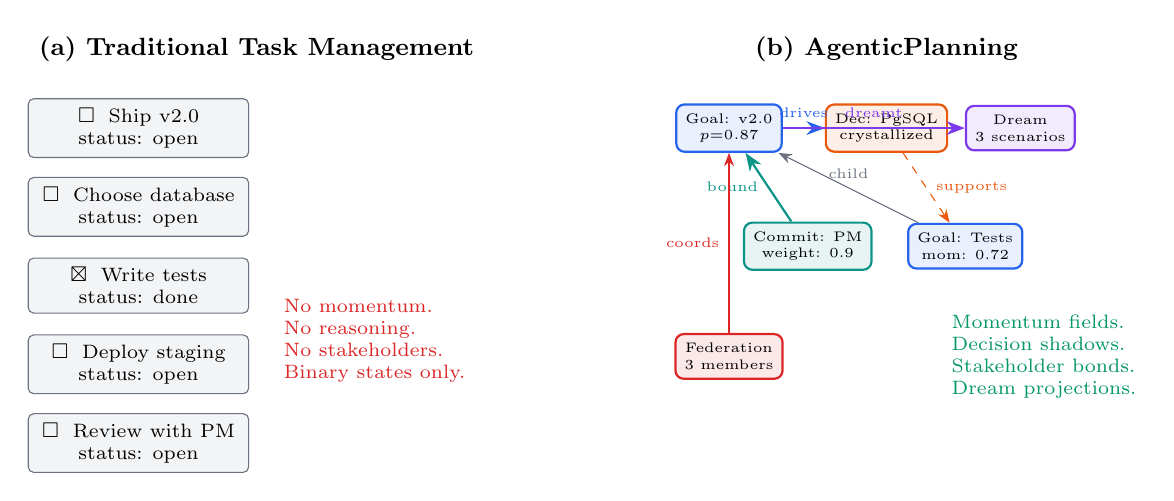
\begin{tikzpicture}[
  node distance=1.2cm,
  every node/.style={font=\small},
  tasknode/.style={rectangle, draw=amgray, fill=amlightgray, rounded corners=2pt, minimum width=2.8cm, minimum height=0.6cm, align=center, font=\scriptsize},
  goalnode/.style={rectangle, rounded corners=3pt, draw=amblue, fill=amblue!10, minimum width=1.1cm, minimum height=0.5cm, font=\tiny, align=center, thick},
  decnode/.style={rectangle, rounded corners=3pt, draw=amorange, fill=amorange!10, minimum width=1.1cm, minimum height=0.5cm, font=\tiny, align=center, thick},
  dreamnode/.style={rectangle, rounded corners=3pt, draw=ampurple, fill=ampurple!10, minimum width=1.1cm, minimum height=0.5cm, font=\tiny, align=center, thick},
  commitnode/.style={rectangle, rounded corners=3pt, draw=amteal, fill=amteal!10, minimum width=1.1cm, minimum height=0.5cm, font=\tiny, align=center, thick},
  fednode/.style={rectangle, rounded corners=3pt, draw=amred, fill=amred!10, minimum width=1.1cm, minimum height=0.5cm, font=\tiny, align=center, thick},
]

% Left side: Traditional Task List
\node[font=\small\bfseries] at (-4.5, 3.2) {(a) Traditional Task Management};

\node[tasknode] (t1) at (-6.0, 2.2) {$\square$\; Ship v2.0\\status: open};
\node[tasknode] (t2) at (-6.0, 1.2) {$\square$\; Choose database\\status: open};
\node[tasknode] (t3) at (-6.0, 0.2) {$\boxtimes$\; Write tests\\status: done};
\node[tasknode] (t4) at (-6.0, -0.8) {$\square$\; Deploy staging\\status: open};
\node[tasknode] (t5) at (-6.0, -1.8) {$\square$\; Review with PM\\status: open};

\node[font=\scriptsize\color{amred}, align=left] at (-3.0, -0.5) {No momentum.\\No reasoning.\\No stakeholders.\\Binary states only.};

% Right side: AgenticPlanning
\node[font=\small\bfseries] at (3.5, 3.2) {(b) AgenticPlanning};

\node[goalnode] (g1) at (1.5, 2.2) {Goal: v2.0\\$p{=}0.87$};
\node[decnode] (d1) at (3.5, 2.2) {Dec: PgSQL\\crystallized};
\node[dreamnode] (dr1) at (5.2, 2.2) {Dream\\3 scenarios};
\node[commitnode] (c1) at (2.5, 0.7) {Commit: PM\\weight: 0.9};
\node[goalnode] (g2) at (4.5, 0.7) {Goal: Tests\\mom: 0.72};
\node[fednode] (f1) at (1.5, -0.7) {Federation\\3 members};

\draw[-{Stealth}, amblue, thick] (g1) -- node[above, font=\tiny, text=amblue] {drives} (d1);
\draw[-{Stealth}, ampurple, thick] (g1) -- node[above, font=\tiny, text=ampurple] {dreamt} (dr1);
\draw[-{Stealth}, amteal, thick] (c1) -- node[left, font=\tiny, text=amteal] {bound} (g1);
\draw[-{Stealth}, amgray] (g2) -- node[above, font=\tiny, text=amgray] {child} (g1);
\draw[-{Stealth}, amred] (f1) -- node[left, font=\tiny, text=amred] {coords} (g1);
\draw[-{Stealth}, amorange, dashed] (d1) -- node[right, font=\tiny, text=amorange] {supports} (g2);

\node[font=\scriptsize\color{amgreen}, align=left] at (5.5, -0.7) {Momentum fields.\\Decision shadows.\\Stakeholder bonds.\\Dream projections.};

\end{tikzpicture}
\caption{Comparison of planning paradigms. (a)~Traditional task management stores goals as flat records with binary open/closed states; no relationships, reasoning provenance, or dynamic properties are preserved. (b)~AgenticPlanning models goals as physical entities with momentum, decisions as crystallized choices with preserved shadows, commitments as stakeholder-bound promises, and dreams as forward projections---all connected by typed relationships.}
\label{fig:comparison}
\end{figure*}


% ============================================================================
% 2. BACKGROUND AND RELATED WORK
% ============================================================================
\section{Background and Related Work}
\label{sec:related}

We survey the primary approaches to planning and goal management for AI agents.

\textbf{Classical AI planning.} STRIPS~\cite{fikes1971strips} and its descendants---PDDL~\cite{mcdermott1998pddl}, HTN planners~\cite{nau2003shop2}, and constraint-based planners~\cite{ghallab2004automated}---model planning as search over symbolic state spaces with predefined operators. These systems excel at well-defined logistics problems but assume complete knowledge of the action space, cannot model ambiguity or stakeholder dynamics, and produce plans that are static artifacts rather than living, evolving structures.

\textbf{Task management systems.} Tools such as Todoist, Linear, and Jira~\cite{jira_2024} provide persistent task tracking with rich metadata (priorities, labels, assignees). However, they model tasks as static database records with binary completion states. There is no mechanism to capture why a goal exists (its ``soul''), how urgent it has become through sustained neglect, what decisions were made in pursuit of it, or what momentum it has accumulated.

\textbf{Agent planning frameworks.} AutoGPT~\cite{autogpt_2024} decomposes high-level objectives into task lists and executes them iteratively. BabyAGI~\cite{babyagi_2024} maintains a priority queue of tasks that the LLM itself reorders. CrewAI~\cite{crewai_2024} introduces role-based agent coordination. These systems generate plans dynamically but store them as ephemeral in-memory or text-file state. No planning history survives session boundaries, and there is no structured model of decisions, commitments, or progress dynamics.

\textbf{Generative agent architectures.} Park et al.~\cite{park2023generative} demonstrated that memory architecture profoundly impacts agent behavior, using a retrieval system combining recency, importance, and relevance scores. Their work reinforces our thesis that planning requires richer dynamic structure, but focuses on memory recall rather than persistent goal management.

\textbf{Plan representation languages.} O-Plan~\cite{currie1991oplan} and SIPE-2~\cite{wilkins1988sipe} introduced hierarchical partial-order planning with temporal constraints. While more expressive than STRIPS, these systems model plans as logical structures without the physical metaphors (momentum, gravity, energy) that we argue better capture the dynamics of intention over time.

Table~\ref{tab:related} summarizes the comparison across key dimensions.

\begin{table*}[t]
\caption{Comparison of planning systems across key dimensions relevant to AI agent deployment.}
\label{tab:related}
\centering
\small
\begin{tabular}{@{}lcccccc@{}}
\toprule
\textbf{System} & \textbf{Persistence} & \textbf{Dynamics} & \textbf{Decisions} & \textbf{Stakeholders} & \textbf{Dependencies} & \textbf{Format} \\
\midrule
PDDL~\cite{mcdermott1998pddl} & None & Static states & N/A & None & Solver & Symbolic \\
Todoist / Linear & Cloud DB & Static records & None & None & Cloud service & Proprietary \\
Jira~\cite{jira_2024} & Cloud DB & Status fields & None & Assignees & Cloud service & Proprietary \\
AutoGPT~\cite{autogpt_2024} & Text files & None & None & None & LLM API & Ephemeral \\
BabyAGI~\cite{babyagi_2024} & In-memory & Priority queue & None & None & LLM API & Ephemeral \\
CrewAI~\cite{crewai_2024} & In-memory & Role-based & None & Agents & LLM API & Ephemeral \\
Park et al.~\cite{park2023generative} & JSON & Recency/import. & None & None & LLM API & Text \\
\midrule
\textbf{AgenticPlanning} & \textbf{Binary file} & \textbf{Physics model} & \textbf{Crystallization} & \textbf{Weighted} & \textbf{None} & \textbf{.aplan} \\
\bottomrule
\end{tabular}
\end{table*}


% ============================================================================
% 3. ARCHITECTURE
% ============================================================================
\section{Architecture}
\label{sec:architecture}

AgenticPlanning models the planning state as a collection of typed entities stored in a \texttt{PlanningEngine} backed by in-memory hash maps and persisted to a single binary file. The engine maintains six entity stores, a set of secondary indexes, an append-only audit log, and a write counter for crash recovery.

% ----------------------------------------------------------------------------
\subsection{Entity Model}
\label{sec:entities}

The system defines six core entity types, each with rich sub-structure:

\begin{itemize}[nosep, leftmargin=*]
  \item \textbf{Goal} --- A living intention with seven sub-components: \emph{soul} (title, description, purpose, values alignment), \emph{feelings} (urgency, neglect, confidence, alignment, vitality), \emph{physics} (momentum, gravity, inertia, energy, velocity), \emph{provenance} (creation context), \emph{metamorphosis} (evolution history), and \emph{karma} (impact record). Goals progress through a lifecycle: \textsc{Seed} $\to$ \textsc{Active} $\to$ \textsc{Completed}/\textsc{Abandoned}/\textsc{Paused}/\textsc{Reincarnated}.
  \item \textbf{Decision} --- A crystallization event modeling the transition from fluid possibility to firm commitment. Each decision contains a \emph{question} framing the choice, multiple \emph{paths} (options with pros, cons, effort, and risk estimates), and upon crystallization, a \emph{reasoning} record (rationale, factors, weights, confidence) plus \emph{crystal shadows}---preserved records of unchosen paths for future archaeology.
  \item \textbf{Commitment} --- An entangled promise to a specific stakeholder. Each commitment binds a \emph{promise} (description, deliverables, conditions) to a \emph{stakeholder} (name, role, importance weight), with optional due dates, entanglement records, and fulfillment tracking.
  \item \textbf{Dream} --- A forward projection of goal completion. Dreams contain \emph{completion scenarios} (narrative, confidence, timeline), \emph{obstacles} (description, severity, mitigation), \emph{insights} (observations, implications, actions), \emph{goal seeds} (new goals discovered during dreaming), and \emph{accuracy} tracking for retrospective calibration.
  \item \textbf{Federation} --- A coordination structure grouping multiple goals under a shared coordinator with member roles.
  \item \textbf{Consensus} --- A collective decision-making record for federated goal groups.
\end{itemize}

All entities are identified by UUID-based typed IDs (\texttt{GoalId}, \texttt{DecisionId}, etc.) and carry creation timestamps. The engine maintains secondary indexes mapping goals to their decisions, commitments, and dreams for efficient cross-entity queries.

% Figure 2: Entity model
\begin{figure}[t]
\centering
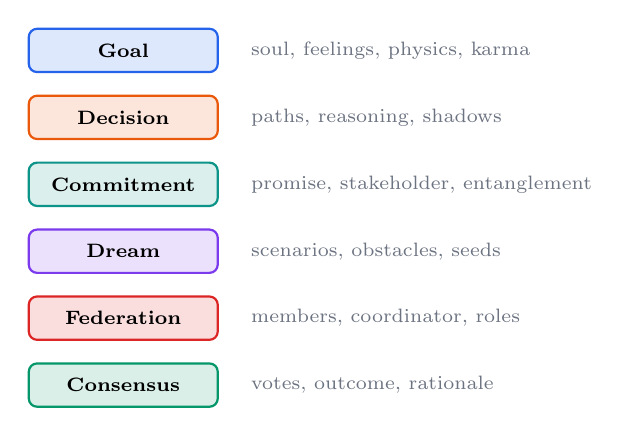
\begin{tikzpicture}[
  every node/.style={font=\scriptsize},
  typebox/.style={rectangle, rounded corners=3pt, minimum width=2.4cm, minimum height=0.55cm, align=center, draw, thick, font=\scriptsize\bfseries},
]
\node[typebox, fill=amblue!15, draw=amblue] (goal) at (0, 0) {Goal};
\node[typebox, fill=amorange!15, draw=amorange] (dec) at (0, -0.85) {Decision};
\node[typebox, fill=amteal!15, draw=amteal] (commit) at (0, -1.70) {Commitment};
\node[typebox, fill=ampurple!15, draw=ampurple] (dream) at (0, -2.55) {Dream};
\node[typebox, fill=amred!15, draw=amred] (fed) at (0, -3.40) {Federation};
\node[typebox, fill=amgreen!15, draw=amgreen] (cons) at (0, -4.25) {Consensus};

\node[anchor=west, font=\scriptsize, text=amgray] at (1.5, 0) {soul, feelings, physics, karma};
\node[anchor=west, font=\scriptsize, text=amgray] at (1.5, -0.85) {paths, reasoning, shadows};
\node[anchor=west, font=\scriptsize, text=amgray] at (1.5, -1.70) {promise, stakeholder, entanglement};
\node[anchor=west, font=\scriptsize, text=amgray] at (1.5, -2.55) {scenarios, obstacles, seeds};
\node[anchor=west, font=\scriptsize, text=amgray] at (1.5, -3.40) {members, coordinator, roles};
\node[anchor=west, font=\scriptsize, text=amgray] at (1.5, -4.25) {votes, outcome, rationale};
\end{tikzpicture}
\caption{The six entity types in AgenticPlanning with their primary sub-components. Goals carry the richest structure with seven sub-component categories modeling the full lifecycle of intention.}
\label{fig:entities}
\end{figure}

% ----------------------------------------------------------------------------
\subsection{Intention Physics}
\label{sec:physics}

The central architectural innovation is modeling goals as physical entities subject to dynamic forces. Each goal carries a \texttt{GoalPhysics} record with five fields:

\begin{itemize}[nosep, leftmargin=*]
  \item \textbf{Momentum} ($p \in [0, 1]$) --- Measures sustained effort. Goals with consistent recent activity accumulate momentum; idle goals see momentum decay. High-momentum goals are more likely to reach completion.
  \item \textbf{Gravity} ($g \in [0, 1]$) --- Measures attractive force. Important goals with many connections (child goals, decisions, commitments) exert stronger gravity, pulling related work toward them.
  \item \textbf{Inertia} ($\iota \in [0, 1]$) --- Resistance to state change. Goals with deep investment resist abandonment; new goals resist activation. This models the sunk-cost dynamics of real planning.
  \item \textbf{Energy} ($E \in [0, 1]$) --- Available cognitive resource. Active goals consume energy; paused goals conserve it. The engine tracks total energy across all active goals to surface overcommitment.
  \item \textbf{Velocity} ($v \in [0, 1]$) --- Rate of progress change. Derived from momentum and recent activity patterns, velocity indicates whether a goal is accelerating or decelerating.
\end{itemize}

These fields are updated by the engine as operations occur (goal activation, decision crystallization, commitment fulfillment) and are surfaced through three aggregate queries: the \emph{momentum report} (per-goal momentum ranking), the \emph{gravity field} (attraction map across all goals), and the \emph{intention singularity} (system-wide coherence metric indicating whether the agent's goals are converging or diverging).

% Figure 3: Intention Physics
\begin{figure}[t]
\centering
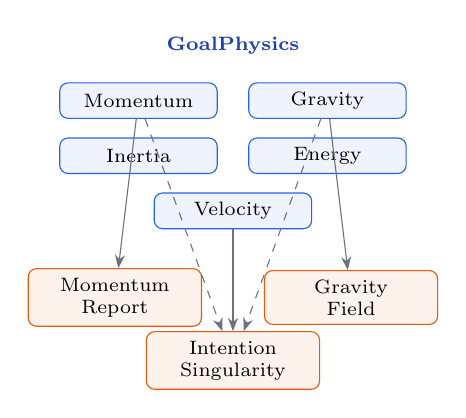
\begin{tikzpicture}[
  every node/.style={font=\scriptsize},
  field/.style={rectangle, rounded corners=3pt, minimum width=2.0cm, minimum height=0.45cm, align=center, draw=amblue, fill=amblue!8, font=\scriptsize},
  query/.style={rectangle, rounded corners=3pt, minimum width=2.2cm, minimum height=0.45cm, align=center, draw=amorange, fill=amorange!8, font=\scriptsize},
]

% Physics fields
\node[font=\scriptsize\bfseries, text=amdarkblue] at (0, 1.2) {GoalPhysics};
\node[field] (mom) at (-1.2, 0.5) {Momentum};
\node[field] (grav) at (1.2, 0.5) {Gravity};
\node[field] (iner) at (-1.2, -0.2) {Inertia};
\node[field] (ener) at (1.2, -0.2) {Energy};
\node[field] (vel) at (0, -0.9) {Velocity};

% Aggregate queries
\node[query] (mrep) at (-1.5, -2.0) {Momentum\\Report};
\node[query] (gfield) at (1.5, -2.0) {Gravity\\Field};
\node[query] (sing) at (0, -2.8) {Intention\\Singularity};

\draw[-{Stealth}, amgray] (mom) -- (mrep);
\draw[-{Stealth}, amgray] (grav) -- (gfield);
\draw[-{Stealth}, amgray] (vel) -- (sing);
\draw[-{Stealth}, amgray, dashed] (mom) -- (sing);
\draw[-{Stealth}, amgray, dashed] (grav) -- (sing);

\end{tikzpicture}
\caption{Intention physics model. Five per-goal fields (momentum, gravity, inertia, energy, velocity) feed three aggregate queries (momentum report, gravity field, intention singularity) that surface system-wide planning dynamics.}
\label{fig:physics}
\end{figure}

% ----------------------------------------------------------------------------
\subsection{Decision Crystallization}
\label{sec:crystallization}

Decisions model the transition from ambiguity to commitment. The lifecycle proceeds in three phases:

\begin{enumerate}[nosep, leftmargin=*]
  \item \textbf{Open} --- The decision exists with a framing question and zero or more paths (options). Each path records a name, description, pros/cons lists, estimated effort ($\in [0,1]$), and estimated risk ($\in [0,1]$).
  \item \textbf{Crystallized} --- The agent selects a path by invoking \texttt{crystallize(id, path\_id, reasoning)}, providing a \texttt{DecisionReasoning} record containing the rationale, factors considered, factor weights, and confidence score. The unchosen paths are preserved as \emph{crystal shadows}---immutable records that enable future decision archaeology (``what did we consider but reject, and why?'').
  \item \textbf{Revisited} --- A crystallized decision can be re-examined, creating an archaeology chain that traces how the agent's decision-making evolved over time.
\end{enumerate}

This model captures an essential property of human planning: decisions are not simple variable assignments but irreversible crystallization events whose full context (including what was \emph{not} chosen) carries information.

% ----------------------------------------------------------------------------
\subsection{Binary File Format}
\label{sec:format}

The \texttt{.aplan} file format is designed for integrity, determinism, and crash safety. The layout consists of three regions:

\begin{itemize}[nosep, leftmargin=*]
  \item \textbf{Header} (128 bytes) --- Magic bytes (\texttt{PLAN}), format version (currently 1), creation and modification timestamps, per-entity counts (goal, decision, commitment, dream, federation), six section offsets pointing into the body, a 32-byte BLAKE3~\cite{blake3_2020} checksum of the body, and 14 reserved bytes.
  \item \textbf{Body} (variable) --- Six JSON-serialized sections, one per entity type. Each section uses \texttt{BTreeMap} ordering (sorted by UUID) to ensure \emph{deterministic serialization}: the same logical state always produces the same byte sequence, enabling reliable checksum verification.
  \item \textbf{Footer} (64 bytes) --- Total file size, monotonic write counter, last session UUID (16 bytes), integrity marker (\texttt{PLANEND\textbackslash{}0}), a 16-byte footer checksum, and 8 reserved bytes.
\end{itemize}

\textbf{Atomic writes.} The save operation writes to a temporary file, calls \texttt{fsync()} to ensure durability, then atomically renames the temporary file over the target path. This guarantees that either the complete new state is visible or the previous state remains intact---the file is never in a partially-written state.

\textbf{Crash recovery.} On \texttt{open()}, the engine checks for orphaned \texttt{.aplan.tmp} files left by an interrupted save. If found, the temporary file is removed and the last complete state is loaded.

\textbf{File locking.} A \texttt{FileLock} guard prevents concurrent writes from multiple processes, ensuring single-writer safety.

\textbf{Integrity verification.} On \texttt{load()}, the engine verifies the magic bytes, format version, integrity marker, and BLAKE3 checksum. A legacy bypass permits loading files written before checksum enforcement (zero-filled checksum fields).

% Figure 4: File format
\begin{figure}[t]
\centering
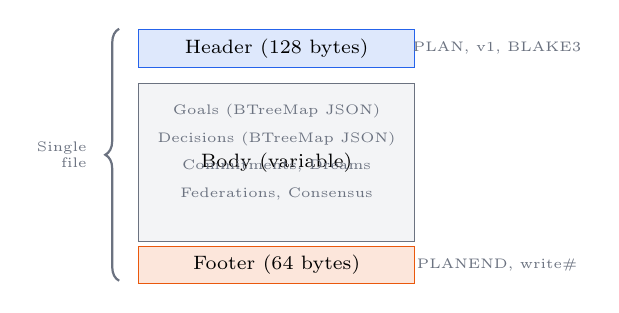
\begin{tikzpicture}[
  every node/.style={font=\scriptsize},
  section/.style={rectangle, minimum width=3.5cm, minimum height=0.45cm, align=center, draw=amgray, font=\scriptsize},
]

\node[section, fill=amblue!15, draw=amblue] (hdr) at (0, 0) {Header (128 bytes)};
\node[font=\tiny, text=amgray, align=left] at (2.8, 0) {PLAN, v1, BLAKE3};

\node[section, fill=amlightgray, minimum height=2.0cm] (body) at (0, -1.45) {Body (variable)};
\node[font=\tiny, text=amgray, align=left] at (0, -0.8) {Goals (BTreeMap JSON)};
\node[font=\tiny, text=amgray, align=left] at (0, -1.15) {Decisions (BTreeMap JSON)};
\node[font=\tiny, text=amgray, align=left] at (0, -1.5) {Commitments, Dreams};
\node[font=\tiny, text=amgray, align=left] at (0, -1.85) {Federations, Consensus};

\node[section, fill=amorange!15, draw=amorange] (ftr) at (0, -2.75) {Footer (64 bytes)};
\node[font=\tiny, text=amgray, align=left] at (2.8, -2.75) {PLANEND, write\#};

\draw[decorate, decoration={brace, amplitude=5pt, mirror}, thick, amgray]
  (-2.0, 0.25) -- (-2.0, -2.95) node[midway, left=8pt, font=\tiny, text=amgray, align=right] {Single\\file};

\end{tikzpicture}
\caption{The \texttt{.aplan} binary file format. A 128-byte header carries magic bytes, version, entity counts, section offsets, and a BLAKE3 checksum. The body contains JSON-serialized entity stores with deterministic BTreeMap ordering. A 64-byte footer provides the integrity marker and write counter.}
\label{fig:format}
\end{figure}

% ----------------------------------------------------------------------------
\subsection{Query Engine}
\label{sec:queries}

The query engine provides both direct entity access and aggregate analytics:

\begin{itemize}[nosep, leftmargin=*]
  \item \textbf{Filtered listing} --- \texttt{list\_goals(GoalFilter)} supports filtering by status, priority, and parent, returning matching goals in constant time per result via hash map iteration.
  \item \textbf{Active goal retrieval} --- \texttt{get\_active\_goals()} returns only goals in the \textsc{Active} state, a hot-path query optimized to 4.4\,\textmu s on 1{,}000~goals.
  \item \textbf{Intention singularity} --- Computes a system-wide coherence metric by aggregating momentum, gravity, and velocity across all active goals. Returned in 731.6\,\textmu s on 1{,}000~goals.
  \item \textbf{Momentum report} --- Ranks all goals by momentum, surfacing which goals have sustained effort and which are stalling. Computed in 23.5\,\textmu s.
  \item \textbf{Gravity field} --- Maps the attractive force landscape across all goals, revealing which goals are pulling the most related work. Computed in 19.2\,\textmu s.
  \item \textbf{Dream generation} --- Forward-projects goal completion via \texttt{dream\_goal(id)}, producing scenarios, obstacles, insights, and potential new goal seeds. Generated at 4.0\,\textmu s per dream.
  \item \textbf{Decision archaeology} --- Traces the crystallization history of decisions, including preserved shadows of unchosen paths.
  \item \textbf{Commitment inventory} --- Aggregates all commitments by stakeholder, status, and risk level.
\end{itemize}

% ----------------------------------------------------------------------------
\subsection{Write Pipeline and Audit}
\label{sec:writes}

All mutations pass through the write engine, which enforces three invariants:

\begin{enumerate}[nosep, leftmargin=*]
  \item \textbf{Dirty tracking} --- Every mutation marks the engine as dirty, ensuring that \texttt{save()} only performs I/O when state has actually changed.
  \item \textbf{Index maintenance} --- Secondary indexes (goal-to-decisions, goal-to-commitments, goal-to-dreams) are updated atomically with each write.
  \item \textbf{Audit logging} --- Every mutation is recorded in an append-only \texttt{AuditLog} with timestamp, session ID, operation name, entity type, entity ID, action type (\textsc{Create}, \textsc{Update}, \textsc{Delete}, \textsc{StatusChange}, \textsc{Crystallize}, \textsc{Fulfill}, \textsc{Break}), success/failure status, and optional detail/error messages. The audit log is persisted with the planning state, providing a complete operation history.
\end{enumerate}


% ============================================================================
% 4. EVALUATION
% ============================================================================
\section{Evaluation}
\label{sec:evaluation}

We evaluate AgenticPlanning across six benchmark suites implemented as Rust integration tests (\texttt{paper\_benchmarks.rs}). All benchmarks run on the release profile with median-of-three (or median-of-five) timing to reduce variance. The full test suite comprises 161~tests with zero failures.

% ----------------------------------------------------------------------------
\subsection{Benchmark Environment}
\label{sec:bench_env}

All benchmarks were executed on an Apple Silicon system running macOS, compiled with \texttt{cargo test --release}. Temporary directories (\texttt{tempfile::tempdir}) isolate file I/O. In-memory engines (\texttt{PlanningEngine::in\_memory()}) are used for pure computation benchmarks to exclude I/O effects.

% ----------------------------------------------------------------------------
\subsection{Save/Load Scaling}
\label{sec:save_scaling}

Table~\ref{tab:save_scaling} reports persistence performance as entity count grows from 10 to 5{,}000~goals. Save time includes JSON serialization with BTreeMap ordering, BLAKE3 checksum computation, and atomic file write (temp + fsync + rename). Load time includes file read, magic/version/integrity verification, BLAKE3 checksum validation, and JSON deserialization.

\begin{table}[t]
\caption{Save/load performance scaling with goal count. Median of 3 runs. File size grows linearly at ${\sim}$1.6\,KB/goal.}
\label{tab:save_scaling}
\centering
\small
\begin{tabular}{@{}rrrrl@{}}
\toprule
\textbf{Goals} & \textbf{Save (ms)} & \textbf{Load (ms)} & \textbf{File (KB)} & \textbf{B/goal} \\
\midrule
10 & 17.2 & 0.09 & 23.2 & 2{,}373 \\
100 & 18.9 & 0.37 & 166.9 & 1{,}709 \\
500 & 15.5 & 1.60 & 806.4 & 1{,}651 \\
1{,}000 & 27.1 & 3.20 & 1{,}605.7 & 1{,}643 \\
5{,}000 & 34.1 & 16.70 & 8{,}008.1 & 1{,}640 \\
\bottomrule
\end{tabular}
\end{table}

File size scales linearly at approximately 1{,}640 bytes per goal at scale, with a modest constant overhead for the 128-byte header, 64-byte footer, and empty entity sections. Save time shows sub-linear growth: 5{,}000~goals (8.0\,MB file) saves in 34.1\,ms, only 2$\times$ the time for 10~goals, because the dominant cost is the atomic rename and fsync, not serialization. Load time scales linearly with file size, as expected for sequential deserialization.

% Save/Load chart
\begin{figure}[t]
\centering
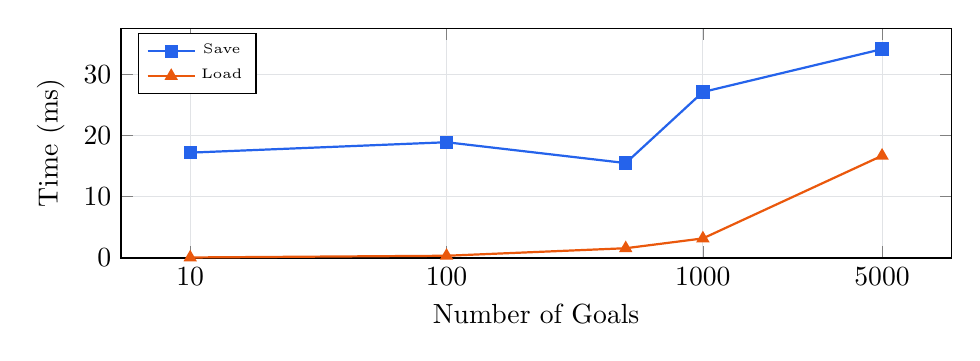
\begin{tikzpicture}
\begin{axis}[
  width=\columnwidth,
  height=4.5cm,
  xlabel={Number of Goals},
  ylabel={Time (ms)},
  legend style={at={(0.02,0.98)}, anchor=north west, font=\tiny},
  grid=major,
  grid style={amgray!20},
  xmode=log,
  log basis x=10,
  ymin=0,
  xtick={10,100,1000,5000},
  xticklabels={10,100,1000,5000},
]
\addplot[color=amblue, mark=square*, thick] coordinates {
  (10, 17.2) (100, 18.9) (500, 15.5) (1000, 27.1) (5000, 34.1)
};
\addlegendentry{Save}
\addplot[color=amorange, mark=triangle*, thick] coordinates {
  (10, 0.09) (100, 0.37) (500, 1.60) (1000, 3.20) (5000, 16.70)
};
\addlegendentry{Load}
\end{axis}
\end{tikzpicture}
\caption{Save and load latency vs.\ goal count. Save time is dominated by fsync/rename overhead, exhibiting sub-linear growth. Load time scales linearly with file size.}
\label{fig:save_load}
\end{figure}

% ----------------------------------------------------------------------------
\subsection{Entity Creation Latency}
\label{sec:creation}

Table~\ref{tab:creation} reports per-operation latency for the three primary entity creation operations, measured over 10{,}000 iterations each on an in-memory engine.

\begin{table}[t]
\caption{Entity creation latency (in-memory engine, 10{,}000 iterations).}
\label{tab:creation}
\centering
\small
\begin{tabular}{@{}lrr@{}}
\toprule
\textbf{Operation} & \textbf{Latency (\textmu s/op)} & \textbf{Total (ms)} \\
\midrule
Goal creation & 1.748 & 17.5 \\
Decision creation & 1.367 & 13.7 \\
Commitment creation & 3.246 & 32.5 \\
\bottomrule
\end{tabular}
\end{table}

Goal and decision creation run below 2\,\textmu s, dominated by UUID generation and hash map insertion. Commitment creation is approximately 2$\times$ slower due to the additional stakeholder construction (UUID generation for StakeholderId plus importance weight normalization).

% ----------------------------------------------------------------------------
\subsection{Query Performance}
\label{sec:query_perf}

Table~\ref{tab:queries} reports query latency on an engine populated with 1{,}000~goals (500 active, mixed priorities), measured over 1{,}000--10{,}000 iterations.

\begin{table}[t]
\caption{Query performance on 1{,}000 goals (500 active).}
\label{tab:queries}
\centering
\small
\begin{tabular}{@{}lrr@{}}
\toprule
\textbf{Query} & \textbf{Latency (\textmu s)} & \textbf{Iterations} \\
\midrule
\texttt{list\_goals} (all) & 10.939 & 10{,}000 \\
\texttt{get\_active\_goals} & 4.377 & 10{,}000 \\
\texttt{intention\_singularity} & 731.636 & 1{,}000 \\
\texttt{momentum\_report} & 23.471 & 1{,}000 \\
\texttt{gravity\_field} & 19.201 & 1{,}000 \\
\bottomrule
\end{tabular}
\end{table}

Direct listing queries (\texttt{list\_goals}, \texttt{get\_active\_goals}) complete in single-digit microseconds, as they iterate over the in-memory hash map with minimal computation per entry. The intention singularity computation is the most expensive query at 731.6\,\textmu s because it aggregates physics fields across all active goals and computes a system-wide coherence metric---still sub-millisecond for 1{,}000 goals. Momentum report and gravity field are intermediate at 19--23\,\textmu s, reflecting per-goal physics calculations without the global aggregation step.

% Query performance chart
\begin{figure}[t]
\centering
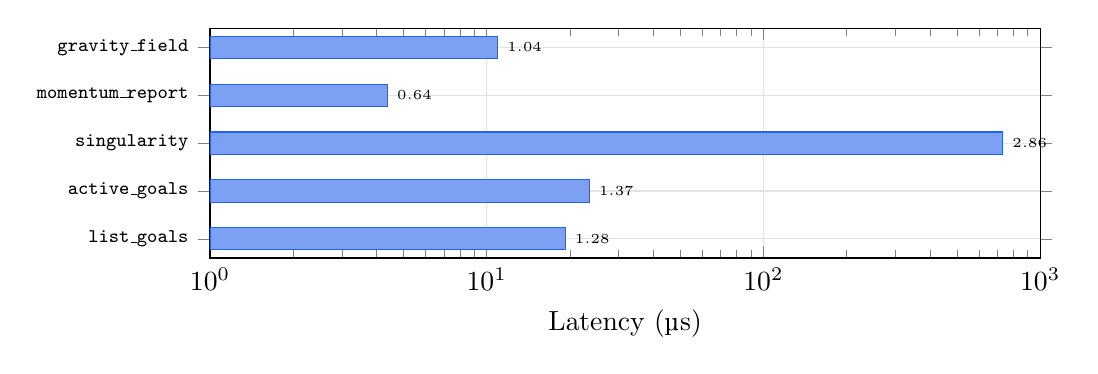
\begin{tikzpicture}
\begin{axis}[
  width=\columnwidth,
  height=4.5cm,
  xbar,
  xlabel={Latency (\textmu s)},
  symbolic y coords={grav, mom, sing, active, listg},
  ytick=data,
  yticklabels={%
    \texttt{gravity\_field},%
    \texttt{momentum\_report},%
    \texttt{singularity},%
    \texttt{active\_goals},%
    \texttt{list\_goals}%
  },
  y tick label style={font=\scriptsize},
  xmode=log,
  log basis x=10,
  xmin=1,
  xmax=1000,
  nodes near coords,
  nodes near coords style={font=\tiny, anchor=west},
  every node near coord/.append style={/pgf/number format/fixed},
  bar width=8pt,
  grid=major,
  grid style={amgray!20},
]
\addplot[fill=amblue!60, draw=amblue] coordinates {
  (10.939,listg)
  (4.377,active)
  (731.636,sing)
  (23.471,mom)
  (19.201,grav)
};
\end{axis}
\end{tikzpicture}
\caption{Query latency on 1{,}000 goals (log scale). Direct listing queries return in $<$11\,\textmu s. Physics aggregations (momentum, gravity) complete in $<$24\,\textmu s. The intention singularity, the most complex aggregate, returns in 731.6\,\textmu s.}
\label{fig:query_perf}
\end{figure}

% ----------------------------------------------------------------------------
\subsection{Dream Generation and Crystallization}
\label{sec:dream_crystal}

Table~\ref{tab:dream_crystal} reports latency for the two most semantically complex operations: dream generation (forward-projecting goal completion scenarios) and decision crystallization (selecting a path with full reasoning).

\begin{table}[t]
\caption{Dream generation and decision crystallization latency.}
\label{tab:dream_crystal}
\centering
\small
\begin{tabular}{@{}lrrr@{}}
\toprule
\textbf{Operation} & \textbf{Latency (\textmu s/op)} & \textbf{Count} & \textbf{Total (ms)} \\
\midrule
Dream generation & 4.036 & 100 & 0.404 \\
Crystallization & 2.627 & 100 & 0.263 \\
\bottomrule
\end{tabular}
\end{table}

Dream generation at 4.0\,\textmu s per dream and crystallization at 2.6\,\textmu s per operation demonstrate that even the most complex semantic operations remain in the low-microsecond range. Crystallization involves selecting a path, copying unchosen paths to shadows, recording the reasoning struct, and updating the decision status---all pure in-memory operations with no I/O.

% ----------------------------------------------------------------------------
\subsection{BLAKE3 Checksum Overhead}
\label{sec:checksum}

Table~\ref{tab:checksum} isolates the cost of integrity verification during save operations. The save time includes serialization, checksum computation, and atomic file write.

\begin{table}[t]
\caption{Save performance with BLAKE3 checksum (median of 5).}
\label{tab:checksum}
\centering
\small
\begin{tabular}{@{}rrrr@{}}
\toprule
\textbf{Goals} & \textbf{Save (ms)} & \textbf{File (KB)} & \textbf{B/goal} \\
\midrule
100 & 18.0 & 159.9 & 1{,}637 \\
500 & 19.6 & 789.5 & 1{,}617 \\
1{,}000 & 26.9 & 1{,}576.7 & 1{,}614 \\
\bottomrule
\end{tabular}
\end{table}

BLAKE3 checksum computation adds negligible overhead: the difference between 100-goal and 1{,}000-goal saves is only 8.9\,ms despite a 10$\times$ increase in data size, confirming that BLAKE3's SIMD-optimized streaming hash~\cite{blake3_2020} contributes minimal latency relative to I/O costs.

% ----------------------------------------------------------------------------
\subsection{System Summary}
\label{sec:sys_summary}

Table~\ref{tab:system} summarizes the implementation metrics.

\begin{table}[t]
\caption{Implementation metrics for AgenticPlanning.}
\label{tab:system}
\centering
\small
\begin{tabular}{@{}lr@{}}
\toprule
\textbf{Metric} & \textbf{Value} \\
\midrule
Production Rust LOC & 17{,}421 \\
Test LOC & 1{,}884 \\
Total LOC & 19{,}305 \\
Crates & 5 \\
Source files & 24 \\
Core entity types & 6 \\
Type definitions & 109 \\
MCP tools & 13 \\
FFI exports & 31 \\
CLI commands & 17 \\
Workspace dependencies & 9 \\
Tests (all passing) & 161 \\
Binary: MCP server & 3.5\,MB \\
Binary: CLI & 6.0\,MB \\
\bottomrule
\end{tabular}
\end{table}


% ============================================================================
% 5. INTEGRATION
% ============================================================================
\section{Multi-Surface Integration}
\label{sec:integration}

AgenticPlanning exposes its capabilities through four complementary surfaces, enabling integration with diverse agent architectures.

% ----------------------------------------------------------------------------
\subsection{Model Context Protocol (MCP)}
\label{sec:mcp}

The MCP server (\texttt{agentic-planning-mcp}, 3.5\,MB binary) implements the Model Context Protocol~\cite{mcp_2024} over JSON-RPC, exposing 13~tools:

\begin{itemize}[nosep, leftmargin=*]
  \item \textbf{Goal management} --- \texttt{create\_goal}, \texttt{activate\_goal}, \texttt{list\_goals}, \texttt{get\_active\_goals}
  \item \textbf{Decisions} --- \texttt{create\_decision}, \texttt{add\_option}, \texttt{crystallize}
  \item \textbf{Commitments} --- \texttt{create\_commitment}
  \item \textbf{Analytics} --- \texttt{intention\_singularity}, \texttt{momentum\_report}, \texttt{gravity\_field}
  \item \textbf{Dreams} --- \texttt{dream\_goal}
  \item \textbf{Persistence} --- \texttt{save}
\end{itemize}

The MCP server supports token-based authentication, graceful shutdown via signal handling (\texttt{SIGINT}, \texttt{SIGTERM}), and per-tool audit logging that records every invocation in the engine's audit trail.

% ----------------------------------------------------------------------------
\subsection{Command-Line Interface}
\label{sec:cli}

The CLI (\texttt{aplan}, 6.0\,MB binary) provides 17~commands covering all engine operations, including interactive goal creation, decision crystallization workflows, and formatted output of analytics queries (momentum report, gravity field, intention singularity). The CLI supports both file-backed and in-memory operation modes.

% ----------------------------------------------------------------------------
\subsection{Foreign Function Interface}
\label{sec:ffi}

The FFI crate (\texttt{agentic-planning-ffi}) exports 31~\texttt{\#[no\_mangle]} C-ABI functions, enabling integration from Python, Node.js, Swift, and any language with C FFI support. Functions follow a consistent pattern: opaque engine handle, JSON-serialized request/response payloads, and explicit memory management via \texttt{free\_string()} for returned allocations.

% ----------------------------------------------------------------------------
\subsection{Sister Bridges}
\label{sec:bridges}

AgenticPlanning includes bridge interfaces for integration with seven sibling systems in the Agentra ecosystem: AgenticMemory (persistent cognitive memory), AgenticVision (visual perception), AgenticCodebase (code graph analysis), AgenticIdentity (cryptographic identity), AgenticTime (temporal reasoning), AgenticComm (inter-agent communication), and AgenticContract (governance contracts). Each bridge defines a trait interface with null-object default implementations, enabling gradual adoption without hard dependencies.


% ============================================================================
% 6. DISCUSSION
% ============================================================================
\section{Discussion}
\label{sec:discussion}

\textbf{Enabled capabilities.} AgenticPlanning makes several operations practical that are impossible with traditional task management. \emph{Intention momentum tracking} surfaces which goals have sustained effort vs.\ which are stalling, enabling agents to reallocate attention. \emph{Gravity field analysis} reveals which goals are attracting the most related work, identifying natural convergence points. \emph{Decision archaeology} through crystal shadows preserves the full context of what was considered and rejected, enabling agents to revisit past decisions with their original reasoning intact. \emph{Dream-based forecasting} projects goal completion scenarios with obstacles and insights, supporting proactive planning. \emph{Commitment entanglement tracking} maintains stakeholder accountability with weighted importance, preventing promises from being silently dropped.

\textbf{The physics metaphor.} Modeling goals as physical entities is not merely an aesthetic choice---it provides a computational framework for reasoning about planning dynamics. Momentum naturally captures the acceleration/deceleration of effort. Gravity captures the attractive force of important goals. Energy conservation surfaces overcommitment. Inertia explains why abandoning deeply-invested goals is difficult. These metaphors translate directly into useful aggregate queries (intention singularity, momentum report, gravity field) that have no analog in binary-state task systems.

\textbf{Deterministic serialization.} The use of BTreeMap ordering for JSON serialization ensures that the same logical state always produces the same byte sequence. This property, combined with BLAKE3 checksums, provides strong integrity guarantees: any bit flip, truncation, or corruption is detected on load. The determinism also simplifies debugging and testing, as file contents are reproducible.

\textbf{Performance characteristics.} The benchmark results reveal that AgenticPlanning's in-memory architecture delivers microsecond-scale operations for all entity creation and query operations. The most expensive operation---intention singularity computation at 731.6\,\textmu s---remains sub-millisecond even on 1{,}000 goals. Save/load performance is dominated by I/O costs (fsync, file read) rather than computation, with BLAKE3 adding negligible overhead. This performance profile is well-suited for interactive agent sessions where operations occur at human-conversation timescales (seconds).

\textbf{Limitations.} The current implementation stores entity bodies as JSON within the binary envelope, limiting compression efficiency compared to a fully binary encoding. The physics model uses normalized $[0,1]$ fields updated by heuristic rules rather than a formal dynamical system; future work could explore differential equation models for more principled dynamics. The engine does not yet support concurrent access from multiple agents; the file lock enforces single-writer semantics. Feature vector search (for semantic goal similarity) is not implemented, as the planning engine operates on structured entities rather than embedding-based retrieval.


% ============================================================================
% 7. CONCLUSION
% ============================================================================
\section{Conclusion}
\label{sec:conclusion}

We have presented AgenticPlanning, a persistent intention-physics engine for AI agent goal management. By modeling goals as physical entities with momentum, gravity, and energy; decisions as crystallization events with preserved shadows; commitments as stakeholder-entangled promises; and dreams as forward projections---AgenticPlanning enables capabilities that flat task management systems cannot provide: intention momentum tracking, gravity field analysis, decision archaeology, dream-based forecasting, and commitment entanglement analysis.

The implementation delivers strong performance in a compact footprint: 17{,}421 lines of production Rust across 5~crates, 161~tests with zero failures, entity creation in 1.4--3.2\,\textmu s, queries in 4.4--731.6\,\textmu s, dream generation at 4.0\,\textmu s, crystallization at 2.6\,\textmu s, and save/load of 5{,}000 goals in 34.1/16.7\,ms with BLAKE3 integrity verification. The entire planning state---potentially months of accumulated goals, decisions, commitments, and dreams---resides in a single portable \texttt{.aplan} file requiring zero external dependencies.

AgenticPlanning is exposed through four complementary surfaces (MCP server with 13~tools, CLI with 17~commands, FFI with 31~exports, and 7~sister bridges), enabling integration with diverse agent architectures. The intention-physics model provides a computational framework for reasoning about planning dynamics that goes beyond the binary open/closed states of traditional task management.

We believe the physics-first approach to planning infrastructure is essential for building agents that can sustain coherent intention over time, reason about the dynamics of their own goals, and maintain accountability to stakeholders across session boundaries. AgenticPlanning represents a step toward agents that do not merely execute tasks but genuinely \emph{plan}.

% ============================================================================
% REFERENCES
% ============================================================================
\bibliographystyle{plain}
\bibliography{references}

\end{document}
